\documentclass{beamer}
\usepackage{graphicx}
\usepackage{amssymb}
\usepackage[encapsulated]{CJK}

\usetheme{Madrid}


\title{Classification}
\subtitle{Cats And Dogs}
\author{Team9}
\date{Presentation , 2019}
\subject{Theoretical Computer Science}

\AtBeginSubsection[]
{
  \begin{frame}<beamer>{Outline}
    \tableofcontents[currentsection,currentsubsection]
  \end{frame}
}


\begin{document}

\begin{frame}
  \titlepage
\end{frame}

\begin{frame}{Outline}
  \tableofcontents

\end{frame}




\section{Introduction}


\begin{frame}{Introduction}{Introduction to your team}
\begin{CJK*}{UTF8}{bsmi}
  \begin{itemize}
  \item {
    1051433 葛東昇  
  }
  \item {
    1051514 沈家葳
  }
  \item {
    1053344 高浩然
  }
  \item {
    1053348 黃世旻
  }
  \end{itemize}
\end{CJK*}
\end{frame}

\begin{frame}{Introduction}{Introduction to the problem you're trying to solve  }
\begin{CJK*}{UTF8}{bsmi}
\begin{itemize}
\item{
我們的這個專題主要要解決的問題是把一張照片讀進來,並且判斷這一張照片是貓還是狗。
}
\end{itemize}
\end{CJK*}
\end{frame}



\section{Methodology}

\begin{frame}{Methodology}{Input of your model }
\begin{CJK*}{UTF8}{bsmi}
  \begin{itemize}
  \item {
我們的網路大腦第一層為torch.nn.conv2D\\
torch.nn.conv2D的輸入為 (N,C\_in,HW)
  }
  \end{itemize}
\end{CJK*}
\end{frame}

\begin{frame}{Methodology}{Output of your model }
\begin{CJK*}{UTF8}{bsmi}
  \begin{itemize}
  \item {
model最後一層為nn.linear(4096,2)
  }
 \item {
nn.linear的outputSize為2
  }
 \item {
故最後輸出的tocrch size為(batch\_size,2)
  }
  \end{itemize}
\end{CJK*}
\end{frame}

\begin{frame}{Methodology}{Each layer of your model}
\begin{CJK*}{UTF8}{bsmi}
\begin{figure}[h]
\begin{center}
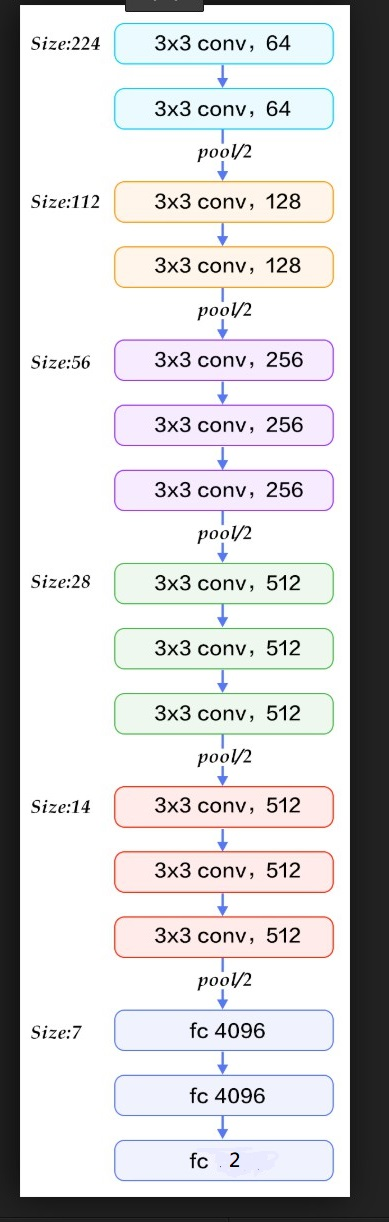
\includegraphics[width=2cm]{Layer.jpg} 
\end{center} 
\label{fig:2} 
\caption{Each Layer} 
\end{figure}
\end{CJK*}
\end{frame}

\begin{frame}{Methodology}{How you save your model?}
\begin{CJK*}{UTF8}{bsmi}
  \begin{itemize}
  \item {
torch.save( )\\
  }
  \end{itemize}
\end{CJK*}  
\end{frame}

\begin{frame}{Methodology}{File size of your model }
\begin{CJK*}{UTF8}{bsmi}
\begin{figure}[h]
\begin{center}
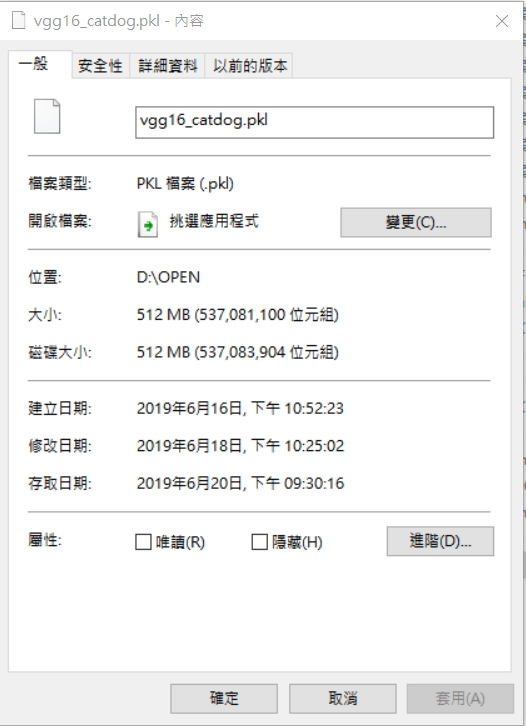
\includegraphics[width=5cm]{model.jpg} 
\end{center} 
\label{fig:1} 
\caption{model size} 
\end{figure}
\end{CJK*}
\end{frame}

\begin{frame}{Methodology}{What's your loss functions, and why? }
\begin{CJK*}{UTF8}{bsmi}
  \begin{itemize}
  \item {
CrossEntropyLoss( )\\
 \item {
torch.nn 用來做圖片分類的最主要有2種\\
NLLLoss跟CrossEntropyLoss\\
但NLLLoss需額外多一層softmax\\
  }
  }
  \end{itemize}
\end{CJK*}
\end{frame}

\begin{frame}{Methodology}{What's your optimizer and the setting of hyperparameter?}
\begin{CJK*}{UTF8}{bsmi}
  \begin{itemize}
  \item {
torch.optim.ASGD
  }
  \end{itemize}
\end{CJK*}
\end{frame}




\section{Dataset}


\begin{frame}{Dataset}{The size of your dataset should be larger than 1K }
\begin{CJK*}{UTF8}{bsmi}
  \begin{itemize}
  \item {
The size of our dataset 大小為26.0MB 共有1200個檔案如圖\\
\begin{figure}[h]
\begin{center}
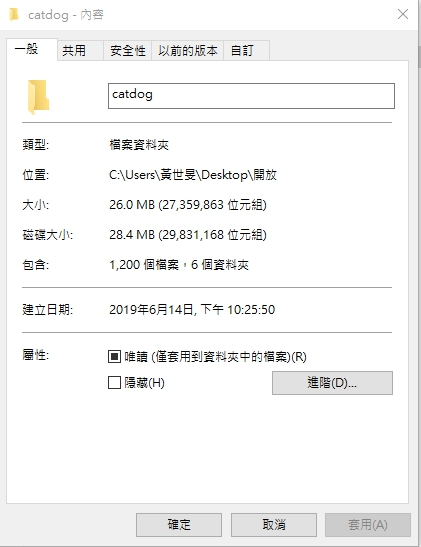
\includegraphics[width=5cm]{dataset.jpg} 
\end{center} 
\label{fig:1} 
\caption{dataset } 
\end{figure}
  }
  \end{itemize}
\end{CJK*}
\end{frame}

\begin{frame}{Dataset}{How you collect/build your dataset?}
\begin{CJK*}{UTF8}{bsmi}
  \begin{itemize}
  \item {
    Collect:train跟validation的部份我們上kaggle抓裡面的圖片下來用,另外test的部分則是我們自己去拍攝。
  }
  \item {
    Build:將照片中間往外開始剪裁224*224,利用torch內建的tramsform,將圖片處理成tensor數據。
  }
  \end{itemize}
\end{CJK*}
\end{frame}

\begin{frame}{Dataset}{How many paired training samples in your dataset?}
\begin{CJK*}{UTF8}{bsmi}
  \begin{itemize}
  \item {
    一共是1000張,貓狗各500張。
  }
  \end{itemize}
\end{CJK*}
\end{frame}

\begin{frame}{Dataset}{How many paired validating samples in your dataset?}
\begin{CJK*}{UTF8}{bsmi}
  \begin{itemize}
  \item {
     一共是200張,貓狗各100張。
  }
  \end{itemize}
\end{CJK*}
\end{frame}

\begin{frame}{Dataset}{How many paired testing samples in your dataset?}
\begin{CJK*}{UTF8}{bsmi}
  \begin{itemize}
  \item {
    一共是20張,貓狗各10張。
  }
  \end{itemize}
\end{CJK*}
\end{frame}




\section{ Experimental Evaluation }

\begin{frame}{ Experimental Evaluation }{Experimental environment}
\begin{CJK*}{UTF8}{bsmi}
  \begin{itemize}
  \item {
    我們所測試的環境是在GPU下進行測試。
  }
  \end{itemize}
\end{CJK*}
\end{frame}

\begin{frame}{ Experimental Evaluation }{How many epochs you set for training?}
\begin{CJK*}{UTF8}{bsmi}
  \begin{itemize}
  \item {
   我們總共設了10個epochs來做training的部分。
  }
  \end{itemize}
\end{CJK*}
\end{frame}

\begin{frame}{ Experimental Evaluation }{Qualitative evaluation }
\begin{CJK*}{UTF8}{bsmi}
\begin{figure}[h]
\begin{center}
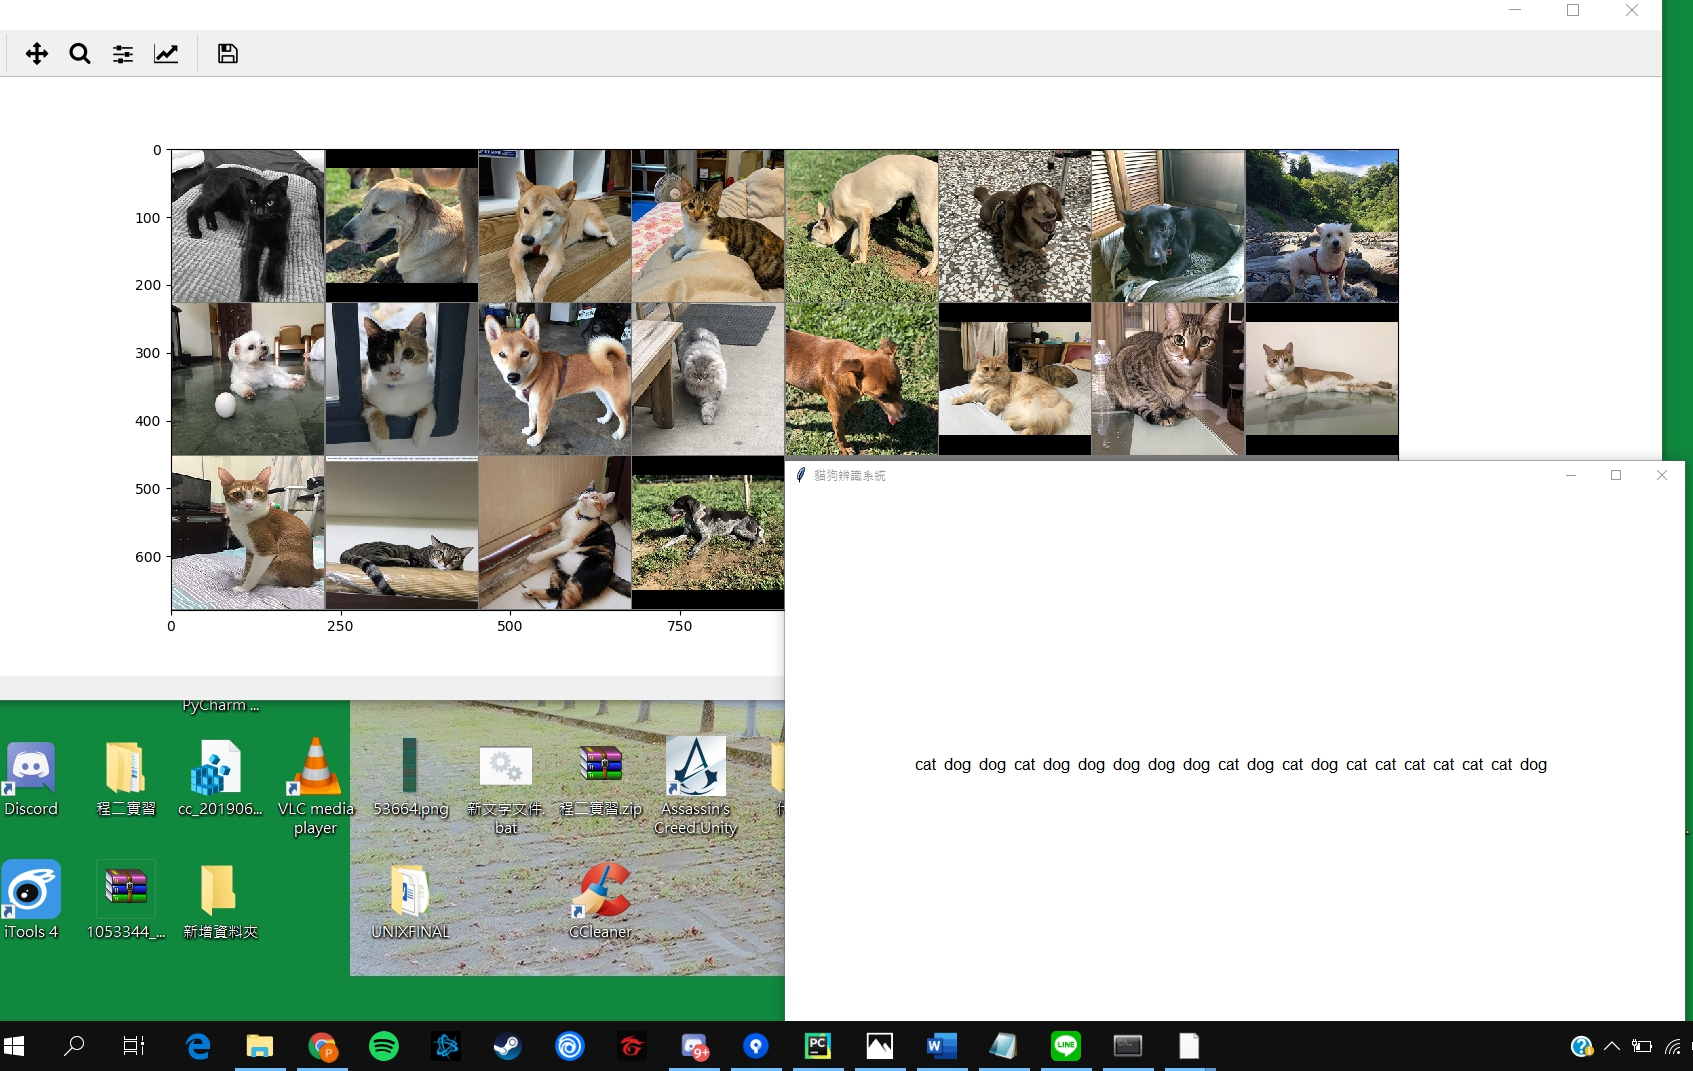
\includegraphics[width=10cm]{eval.jpg} 
\end{center} 
\label{fig:1} 
\caption{質化圖} 
\end{figure}
\end{CJK*}
\end{frame}

\begin{frame}{ Experimental Evaluation }{Quantitative evaluation }
\begin{CJK*}{UTF8}{bsmi}
\begin{figure}[h]
\begin{center}
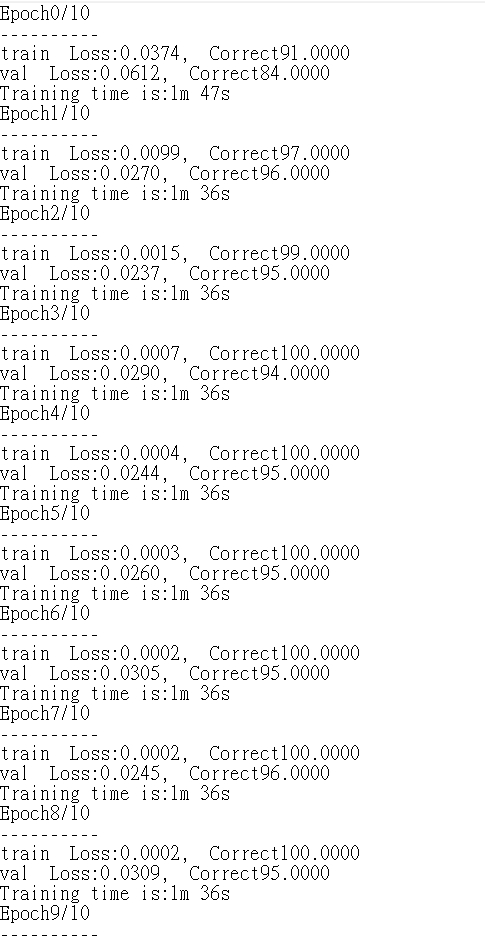
\includegraphics[width=3cm]{qua.jpg} 
\end{center} 
\label{fig:1} 
\caption{量化圖} 
\end{figure}
\end{CJK*}
\end{frame}

\section{Authorship}

\begin{frame}{Authorship}{Cooperate}
\begin{CJK*}{UTF8}{bsmi}
\begin{figure}[h]
\begin{center}
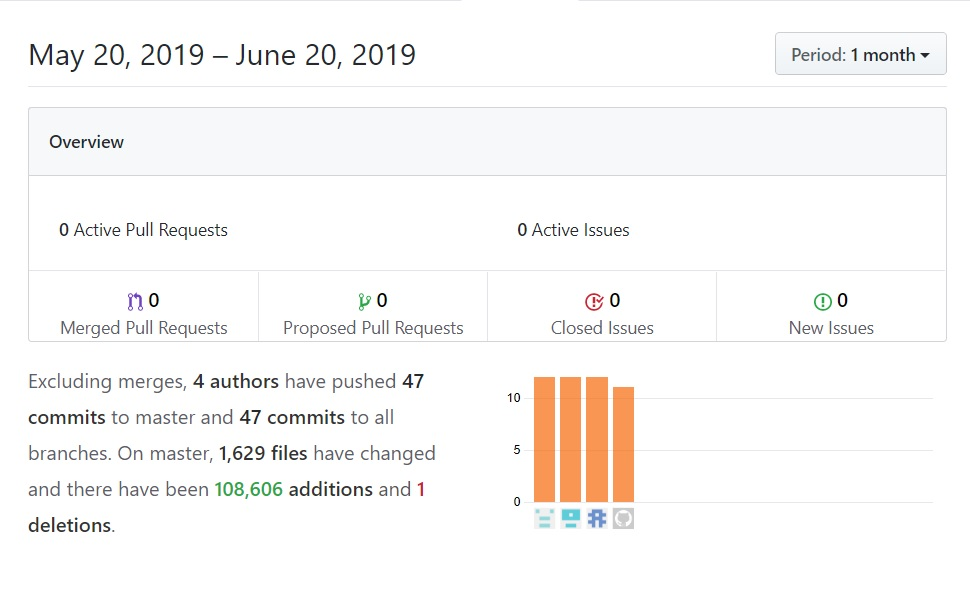
\includegraphics[width=10cm]{Github.jpg} 
\end{center} 
\label{fig:1} 
\caption{GitHub} 
\end{figure}
\end{CJK*}
\end{frame}

\begin{frame}{Authorship }{Job Scheduling }
\begin{CJK*}{UTF8}{bsmi}
\begin{itemize}
  \item{
   6/6 開始蒐集Train Data
}
  \item {
  6/7 開始撰寫程式
  }
  \item {
   6/10 開始撰寫SRS
  }
 \item{
  6/10 開始撰寫PPT
}
\item{
 6/16 修改程式
}
\item{
 6/18 新增GUI
}
\item{
 6/18 SRS完成
}
\item{
 6/20 新增 PPT Authorship 
}
  \end{itemize}
\end{CJK*}
\end{frame}

\begin{CJK*}{UTF8}{bsmi}
\begin{frame}{Authorship }{工作分配}
\begin{itemize}
  \item{
   20\% 資料蒐集
	\begin{itemize}
  	\item{
		1051433  5\%
           }
	\item{
		1051514  5\%
           }
	\item{
		1053344  5\%
           }
	\item{
		1053348  5\%
           }
 	 \end{itemize}
}
  \item {
  30\% 程式Code
	\begin{itemize}
  	\item{
		1051433  20\%
           }
	\item{
		1053348  10\%
           }
 	 \end{itemize}
  }
  \item {
   25\% SRS文件
	\begin{itemize}
	\item{
		1051514  10\%
           }
	\item{
		1053344  10\%
           }
	\item{
		1053348  5\%
           }
 	 \end{itemize}
  }
 \item{
  25\% PPT部分
	\begin{itemize}
	\item{
		1051514  10\%
           }
	\item{
		1053344  10\%
           }
	\item{
		1053348  5\%
           }
 	 \end{itemize}	
}
 \end{itemize}
\end{frame}
\end{CJK*}

\begin{CJK*}{UTF8}{bsmi}
\begin{frame}{Authorship }{工作貢獻表}
\begin{itemize}
  \item{
  1051433   25\%
}
  \item {
  1051514   25\%
  }
  \item {
  1053344   25\%
  }
 \item{
 1053348   25\%
}
 \end{itemize}

\end{frame}
\end{CJK*}
\end{document}


